%!TEX root = /Users/ego/Boulot/TKZ/tkz-graph/doc-fr/TKZdoc-gr-main.tex
% $Id$

%<--------------------------------------------------------------------------->
%                             Vertices
%<--------------------------------------------------------------------------->

\section{Placement de sommets sur une forme géométrique}
Il s'agit ici de placer un groupe de sommets suivant une direction donnée ou bien encore suivant une forme prédéfinie. Les sommets sont placés avec comme support une figure géométrique simple. La macro principale utilise une direction  définie à l'aide de l'option dir, la version étoilée une forme particulière triangulaire, carrée etc...   


\begin{NewMacroBox}{Vertices}{\oarg{local options}\var{type}\var{List of vertices}}
\emph{Il y a donc plusieurs types de formes géométriques, droite, triangle, carrés et cercles. La macro \tkzcname{SetGraphUnit} permet de modifier les  longueurs. Pour les sommets alignés, ceux-ci sont placés suivant une direction donnée par |EA|, |WE|, |NO|, |SO|, |NOEA|, |NOWE|, |SOEA|, |SOWE|.} 

\medskip
\begin{tabular}{llc}
 \toprule
Premier Argument   &            & Définition            \\
\midrule 
\TAline{line  } {} {Sommets alignés, une option détermine la direction} 
\TAline{tr1   } {} {première forme de triangle}   
\TAline{tr2   } {} {deuxième forme de triangle}  
\TAline{tr3   } {} {troisième forme de triangle}  
\TAline{tr4   } {} {quatrième forme de triangle}  
\TAline{square} {} {quatre sommets sur un carré}  
\TAline{circle} {} {sommets sur une cercle}  
\bottomrule
\end{tabular}

\medskip    
\emph{Le second argument est une liste de noms pour les sommets.} 

\medskip    
\begin{tabular}{llc}
\midrule
Options   & Défaut  &      Définition  \\
\midrule
\TOline{dir}  {EA} {permet de placer plusieurs sommets alignés} 
\bottomrule
\end{tabular}

\medskip    
\emph{Les options  sont celles d'un sommet (Vertex).} 
\end{NewMacroBox}    
 

                                                                    
\subsection{\tkzcname{Vertices} à partir d'un sommet défini par des coordonnnées}                 
  
                                                                   
\begin{center}                                                     
\begin{tkzexample}[latex=7cm, ,small]                              
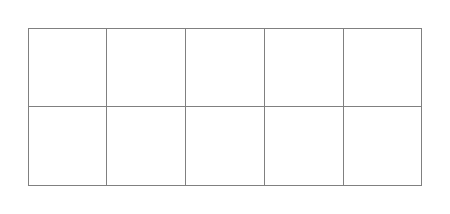
\begin{tikzpicture}
    \SetGraphUnit{2}                       
   \draw[help lines] (0,0) grid (5,2);
   \Vertices[x=1,y=2]{line}{A,B,C}
\end{tikzpicture}
\end{tkzexample}
\end{center}

\subsection{\tkzcname{Vertices} à partir d'une position donnée.}

\begin{center}                                                     
\begin{tkzexample}[latex=7cm, ,small] 
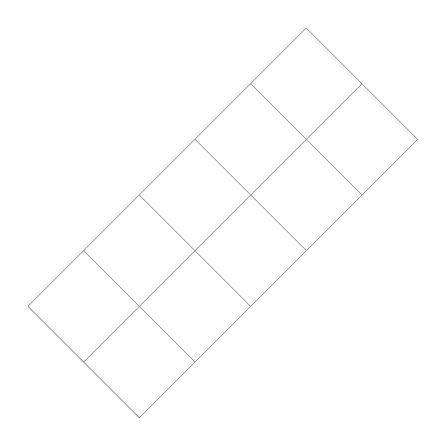
\begin{tikzpicture}[rotate=45] 
  \SetGraphUnit{2}
   \draw[help lines] (0,0) grid (5,2);
   \coordinate (A) at (1,1); 
   \Vertices[Node]{line}{A,B,C}
\end{tikzpicture}
\end{tkzexample}
\end{center}

\subsection{Exemples avec une direction } 
 Il s'agit ici de placer une liste de sommets suivant une direction donnée, cette direction est définie à l'aide de l'option \tkzname{dir}.  


\begin{center}
\begin{tkzexample}[latex=7cm, ,small]  
\begin{tikzpicture}
  \GraphInit[vstyle=Art]
  \Vertices[dir=\NOEA]{line}{A,B,C,D}
  \Vertices[dir=\NOWE]{line}{A,E,F,G}
\end{tikzpicture}
\end{tkzexample}
\end{center} 
              

\subsection{Placement sur un triangle }

Il y a différentes possibilités avec une forme triangulaire, mais les triangles sont isocèles rectangles. Voici dans l'ordre les formes \tkzname{tr1}, \tkzname{tr2} , \tkzname{tr3} et \tkzname{tr4}


\begin{tkzexample}[latex=8cm,small]  
\begin{tikzpicture}\SetGraphUnit{2}
     \Vertices{tr1}{A,B,C}
\end{tikzpicture}\hspace*{2cm}
\begin{tikzpicture}\SetGraphUnit{2}
     \Vertices{tr2}{A,B,C}
\end{tikzpicture}
\end{tkzexample}

\begin{tkzexample}[latex=8cm,small]  
\begin{tikzpicture}\SetGraphUnit{2}
     \Vertices{tr3}{A,B,C}
\end{tikzpicture}\hspace*{2cm}
\begin{tikzpicture}\SetGraphUnit{2}
     \Vertices{tr4}{A,B,C}
\end{tikzpicture}
\end{tkzexample}  


\subsection{Utilisation d'un carré}

 
Deux autres possibilités de placer un node. La première utilise un node obtenu à l'aide d'une intersection (voir le pgfmanual). Dans la première, j'ai redéfini la distance unité entre deux sommets à l'aide de   \tkzcname{SetGraphUnit}.

\begin{center}
\begin{tkzexample}[latex=7cm,small]
\begin{tikzpicture}
   \SetGraphUnit{3}
   \GraphInit[vstyle=Shade]
   \Vertices{square}{A,B,C,D}
   \coordinate (E) at (intersection of A--C and B--D);
   \Vertex[Node]{E}% voir option node
\end{tikzpicture}
\end{tkzexample}
\end{center}


\subsection{Utilisation d'un cercle }

\begin{tkzexample}[latex=7cm,small]  
\begin{tikzpicture}
  \SetGraphUnit{2}
  \Vertices{circle}{A,B,C,D}
\end{tikzpicture}
\end{tkzexample} 


\subsection{Utilisation d'un cercle  et positionnement des labels }

\begin{tkzexample}[latex=7cm,small]   
\begin{tikzpicture} \SetGraphUnit{2}
  \GraphInit[vstyle=Classic]
  \Vertices{circle}{A,B,C,D,E,F}
\end{tikzpicture}
\end{tkzexample}



\subsection{Rotation  et labels externes }

|Lpos| = \tkzname{angle de la rotation}. Cela permet de faire une rotation du label autour du centre de chaque sommet et de suivre la rotation du graphe. Il suffit pour comprendre cette option de compiler l'exemple en l'omettant.  


\begin{tkzexample}[latex=7cm,small] 
\begin{tikzpicture}[rotate=90]
  \GraphInit[vstyle=Classic]
  \Vertices[Lpos=90,unit=2]{circle}{A,B,C,D,E,F}
\end{tikzpicture}
\end{tkzexample}


\subsection{Placement sur un cercle }

Avec des labels externes, il faut procéder avec précaution. 

\begin{tkzexample}[latex=7cm,small] 
\begin{tikzpicture}[scale=.5]
 \SetGraphUnit{4}
 \GraphInit[vstyle=Classic] 
 \begin{scope}[rotate=45] 
   \Vertices[Lpos=45]{circle}{C,E,A,B} 
 \end{scope} 
 \NOEA[Lpos=90,unit=2.828](E){D} 
 \Edges(A,B,E,D,C,E,A,C,B) 
\end{tikzpicture}
\end{tkzexample}

  

\endinput
